\section{Planning the architecture}

While in the planning phase of the project we first planned for making a framework that was to
encompass too much of the tasks of the Android app. We also had a splitting of the framework into
Arduino-to-Framework through wireless connection and another part that was to do the actual fetching
of social service data. This can be found in appendix \ref{app:firstdraftarchi}
After careful consultation with the customer we decided to revise this plan. This was not a heavy blow
to the process as most of our working code was still usable in the new approach. The biggest difference
in the new plan is that the framework or API on Android will communicate with external Android apps through intents,
and the API will then forward this communication through Bluetooth to the Arduino. Intents will be explained
in the documentation and diagrams of this chapter.

\newpage
\section{Architecture diagram}
todo: bla bla ?
\begin{figure}[hb!]
\centering 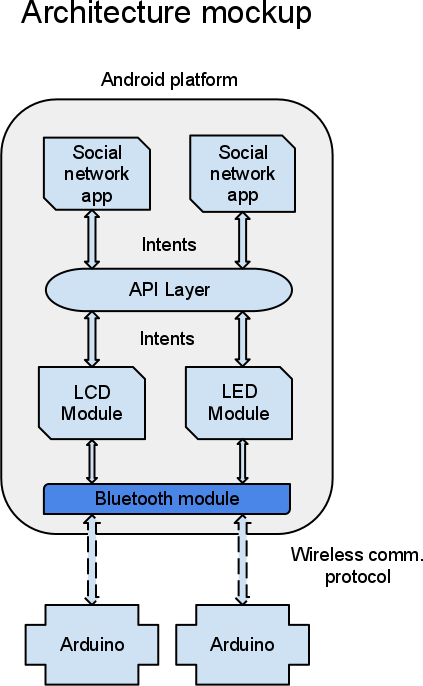
\includegraphics[scale=0.50]{img/architecture.png}
\caption{System architecture}
\label{fig:architecture}
\end{figure}

\section{Use cases}
todo: add use case diagrams